\documentclass[12pt, aspectratio=169]{beamer}
\usepackage[utf8]{inputenc}
\usepackage[T1]{fontenc}
\usepackage{lmodern}
\usepackage[spanish, es-nodecimaldot]{babel}
\uselanguage{spanish}
\languagepath{spanish}
\usepackage{amsmath}
\usepackage{amsfonts}
\usepackage{amssymb}
\usepackage{siunitx}
\usepackage{graphicx}
\usepackage{subcaption}
\usepackage{ragged2e}
\renewcommand{\arraystretch}{1.2}
\author{Alvaro Barreto}
\useinnertheme{rounded} %rectangles, rounded, inmargin, circles
\usetheme{Dresden} %Hannover AnnArbor CambridgeUS Dresden
%\usecolortheme{seahorse}

\makeatletter
\setbeamertemplate{footline}
{
	\leavevmode%
	\hbox{%
		\begin{beamercolorbox}[wd=.333333\paperwidth,ht=2.25ex,dp=1ex,center]{author in head/foot}%
			\usebeamerfont{author in head/foot}\insertshortauthor
		\end{beamercolorbox}%
		\begin{beamercolorbox}[wd=.333333\paperwidth,ht=2.25ex,dp=1ex,center]{title in head/foot}%
			\usebeamerfont{title in head/foot}\insertshorttitle
		\end{beamercolorbox}%
		\begin{beamercolorbox}[wd=.333333\paperwidth,ht=2.25ex,dp=1ex,right]{date in head/foot}%
			\usebeamerfont{date in head/foot}\insertshortdate{}\hspace*{2em}
			\insertframenumber{} / \inserttotalframenumber\hspace*{2ex} 
	\end{beamercolorbox}}%
	\vskip0pt%
}
\makeatother

\setbeamertemplate{blocks}[rounded][shadow=false]
\definecolor{LightViolet}{RGB}{230,220,255}
\setbeamercolor{frametitle}{bg=LightViolet}

\definecolor{NormalBlue}{RGB}{200,200,255}
\setbeamercolor{block title}{bg=NormalBlue}

\definecolor{LightBlue}{RGB}{220,220,255}
\setbeamercolor{block body}{bg=LightBlue}

\setbeamercolor{block body example}{bg=red!20!white}
\setbeamercolor{block title example}{fg=red, bg=red!40!white}

\newcommand{\col}{\column{0.5\textwidth}}
\newcommand{\just}{\justifying}

\begin{document}
	\title{Determinaci\'on del potencial h\'idrico}
	\subtitle{M\'etodo gravim\'etrico}
	\titlegraphic{
		\includegraphics[width=3.5cm]{ENES}
	}
	
	\begin{frame}[plain]
		\titlepage
	\end{frame}

	\begin{frame}{Introducci\'on}
	
		\begin{itemize}
			\item \textbf{\textquestiondown Cu\'al es la funci\'on del agua en la fisiolog\'ia de una planta?}
			\item \onslide<2->{Entre sus principales funciones est\'a el transporte y distribuci\'on de nutrientes y metabolitos en la planta.}
			\item \onslide<3->{\textbf{\textquestiondown El agua puede ser considerada un nutriente?}}
			\item \onslide<4->{S\'i, porque es la forma en que las plantas absorben y asimilan los \'atomos de hidr\'ogeno durante la fotos\'intesis.}
		\end{itemize}
			
	\end{frame}

	\begin{frame}{Movimiento del agua}
		El alcance de una molécula de agua para moverse entre un sistema particular es el \textbf{potencial qu\'imico ($\mu$)}
		
		$$\mu = \frac{\Delta G}{\Delta n}$$
		
	\end{frame}

	\begin{frame}{$\Psi$}
		El potencial h\'idrico ($\Psi$) se deriva de el potencial qu\'imico.
		La conexi\'on entre $\mu$ y $\Psi$ es:
		
		$$\Psi = \frac{\mu_w - \mu_w^{*}}{V} $$ 
		
		\begin{itemize}
			\item $\Psi = $ es el potencial h\'idrico;
			\item  $\mu_w = $ el potencial qu\'imico del agua en el sistema bajo consideraci\'on;
			\item $\mu_w^{*} = $ potencial qu\'imico del agua pura en las mismas condiciones que el sistema en consideraci\'on;
			\item $V = $ volumen molar del agua (18 cm$^3$/mol).
		\end{itemize}
		
	\end{frame}

	\begin{frame}{$\Psi$}
		$\Psi$ incrementa por: 
		\begin{itemize}
			\item Desarrollo de presi\'on hidrost\'atica (turgencia);
			\item Incremento de temperatura.
		\end{itemize}
		
		$\Psi$ disminuye por: 
		\begin{itemize}
			\item Adici\'on de s\'olidos;
			\item Fuerzas m\'atricas que adsorben agua;
			\item Presi\'on negativa;
			\item Reducci\'on de temperatura.
		\end{itemize}
				
	\end{frame}

	\begin{frame}{Componentes de $\Psi$}
		En un sistema particular, el potencial h\'idrico puede ser expresado como la suma de cuatro componentes:
		
		$$\Psi = \Psi_p + \Psi_s + \Psi_m + \Psi_g$$
		
		\only<2>{$\Psi_p = $ potencial de presi\'on. Es el resultado de la presi\'on hidrost\'atica en la c\'elula, que ocurre cuando la presi\'on celular equilibra la diferencia de potencial hídrico entre el ambiente que rodea a la célula y el citoplasma}
		
		\only<3>{$\Psi_s = $ potencial osm\'otico. Es consecuencia a la presi\'on de solutos disueltos, disminuye la energ\'ia del agua y siempre es negativo}
		
		\only<4>{$\Psi_m = $ potencial m\'atrico. Es producto de fuerzas en las superficies de los s\'olidos. Su principal contribuci\'on es la fuerzas que retienen las mol\'eculas de agua por capilaridad, adsorci\'on e hidrataci\'on, en la superficie de las paredes celulares y el citoplasma}
		
		\only<5>{$\Psi_g = $ componente gravitacional. Es producto de la diferencia en energ\'ia potencial como resultado de la diferencia en altura con el nivel de referencia. Por lo general aumenta 0.01 MPa/m por encima del nivel del suelo}
		
	\end{frame}

	\begin{frame}{$\Psi$ con dos componentes}
		
		El potencial h\'idrico puede ser definido como: 
		
		$$\Psi = \Psi_p + \Psi_s$$
						
	\end{frame}

	\begin{frame}{Gradiente del $\Psi$}
		
		\begin{figure}
			\includegraphics[width=\textwidth]{Gradiente_potencial}
			\centering
			%\caption{\textit{Diagrama en el que se ilustran las contribuciones del potencial osmótico ($\Psi_s$), el potencial de presión ($\Psi_p$ ) y el potencial hídrico ($\Psi$) al movimiento del agua entre las células. Los valores de $\Psi$ se expresan en MPa.}}
			\label{fig:gradiente}
		\end{figure}
		
	\end{frame}

	\begin{frame}{C\'alculo  de $\Psi_s$}
		
		La forma de calcular $\Psi_s$ para muchas soluciones biol\'ogicas es con la relaci\'on de van't Hoff:
		
		$$ \Psi_s = -C i R T$$
		
		\begin{itemize}
			\item $C = $ concentraci\'on de soluto expresada en moles
			\item $i = $ constante de ionizaci\'on, para la sacarosa es igual a 1
			\item $R = $ constante de gases, su valor es 0.00831 Kg MPa/mol/K
			\item $T = $ Temperatura en grados Kelvin ($^\circ$C + 273) 
		\end{itemize}
		
	\end{frame}

	\begin{frame}{Medici\'on del potencial h\'idrico}
		\framesubtitle{M\'etodo gravim\'etrico}
		Las c\'elulas vegetales ajustan constantemente su estado h\'idrico a consecuencia de los cambios en el contenido de agua del entorno y a variaciones del estado metab\'olico.
	\end{frame}

	\begin{frame}
		\begin{figure}
			\includegraphics[width=200px]{Plasmolisis}
			\centering
			%\caption{\textit{Estado de la c\'elula cuando se encuentra en diferentes condiciones del medio extracelular.}}
			%\label{fig:pasmolisis}
		\end{figure}
	\end{frame}

	\begin{frame}
		De este modo cuando un tejido se sumerge en soluciones con potencial osm\'otico conocido estos cambiaran su peso, ya que el volumen celular cambia dependiendo de la concentraci\'on osm\'otica de la soluci\'on. Por lo tanto, en est\'a pr\'actica vamos a conocer el potencial osm\'otico de la papa \textit{Solanum tuberosum} para estimar el punto isosmotico.
	\end{frame}

	\begin{frame}{Objetivos}
		\begin{enumerate}
				
			\item Determinar el peso de los tejidos en papa \textit{Solanum tuberosum} con diferentes soluciones de sacarosa. 
				
			\item Evaluaci\'on del potencial h\'idrico en tejidos de papa \textit{Solanum tuberosum}.
			
		\end{enumerate}
	
	\end{frame}

	\begin{frame}{Procedimiento}
		
		La cantidad de sacarosa para preparar 100 mL de soluci\'on en las siguientes concentraciones molares.
		
		\begin{tabular}{p{0.33\textwidth}p{0.33\textwidth}p{0.33\textwidth}}
			0.05 M = 1.71 g  &  0.25 M = 8.56 g & 0.5 M = 17.12 g \\
			0.1 M = 3.42 g & 0.3 M = 10.27 g & \underline{0.7 M = 23.96 g} \\
			0.2 M = 6.85 g & 0.4 M = 13.69 g & \underline{0.8 M = 27.38 g}
		\end{tabular}
		
	\end{frame}

	\begin{frame}
	
		\begin{figure}
			\includegraphics[width=400px]{1.png}
			\centering
		\end{figure}
	
	\end{frame}

	\begin{frame}
		
		\begin{figure}
			\includegraphics[width=400px]{2_.png}
			\centering
		\end{figure}
		
	\end{frame}

	\begin{frame}
		
		\begin{figure}
			\includegraphics[width=400px]{3.png}
			\centering
		\end{figure}
		
	\end{frame}

	\begin{frame}
		
		\begin{figure}
			\includegraphics[width=400px]{4.png}
			\centering
		\end{figure}
		
	\end{frame}

	\begin{frame}
	
		\begin{figure}
			\includegraphics[width=400px]{5.png}
			\centering
	\end{figure}
	
	\end{frame}

	\begin{frame}
		\tiny 
		\begin{table}
			 
			\caption{Datos de cambio de peso en porciones de papa incubadas en diferentes soluciones de sacarosa.}
			
			\label{resultados:potencial}
			\centering
			\begin{tabular}{|p{0.17\textwidth}|p{0.17\textwidth}|p{0.17\textwidth}|p{0.17\textwidth}|p{0.17\textwidth}|}
				
				\hline  &&&& \\
				Soluci\'on sacarosa (M) & Peso inicial (g) & Peso final (g) & $\Delta$ peso$^\dagger$ (g) & Porcentaje $\Delta$ peso$^\mp$ \\
				&&&& \\
				\hline 
				0.00 &&&& \\
				0.05 &&&& \\
				0.10 &&&& \\
				0.20 &&&& \\
				0.25 &&&& \\
				0.30 &&&& \\
				0.40 &&&& \\
				0.50 &&&& \\
				%0.70 &&&& \\
				%0.80 &&&& \\
				
				\hline 
				
				\multicolumn{5}{l}{\footnotesize $^\dagger$ $\Delta$ peso = Peso final - Peso inicial. } \\
				\multicolumn{5}{l}{\footnotesize $^\mp$ Porcentaje $\Delta$ peso = $\Delta$ peso / Peso inicial. }	
			
			\end{tabular}
		\end{table}
	\end{frame}

	\begin{frame}
			\includegraphics[width=250px]{graf_cambio.png}
		\centering
	\end{frame}

	\begin{frame}{C\'alculo  de $\Psi_s$}
		
		La forma de calcular $\Psi_s$ para muchas soluciones biol\'ogicas es con la relaci\'on de van't Hoff:
		
		$$ \Psi_s = -C i R T$$
		
		\begin{itemize}
			\item $C = $ concentraci\'on de soluto expresada en moles
			\item $i = $ constante de ionizaci\'on, para la sacarosa es igual a 1
			\item $R = $ constante de gases, su valor es 0.00831 Kg MPa/mol/K
			\item $T = $ Temperatura en grados Kelvin ($^\circ$C + 273) 
		\end{itemize}
		
	\end{frame}

\end{document}